\documentclass[tikz,border=3pt]{standalone}
\usepackage[utf8]{inputenc}
\usepackage[T1]{fontenc}
\usepackage{libertinus}
\usepackage{amsmath,amssymb}
\usetikzlibrary{arrows.meta,calc,patterns,decorations.pathmorphing,decorations.markings,decorations.pathreplacing,bending}
\definecolor{UGblue}{RGB}{0,51,102}
\newcommand{\dbar}{\mathchar'26\mkern-12mu d}
\tikzset{
  >=Stealth,
  every node/.style={font=\small},
  caja/.style={draw,line width=0.9pt},
  pared/.style={draw,line width=1.6pt},
  ejes/.style={->,line width=0.8pt},
  adia/.style={draw,pattern=north east lines,pattern color=black!70,line width=0.5pt},
  gas/.style={fill=UGblue!8},
  punto/.style={fill,circle,inner sep=1.3pt},
  onda/.style={decorate,decoration={snake,amplitude=1.1pt,segment length=5pt,post length=3pt,pre length=0pt}},
}
\begin{document}
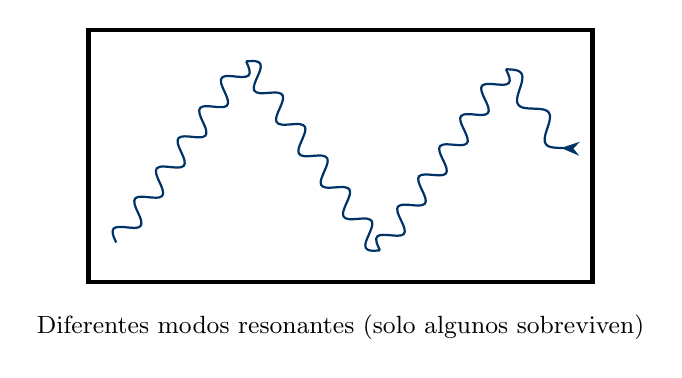
\begin{tikzpicture}
  \draw[pared] (0,0) rectangle (6.4,3.2);
  \draw[line width=0.8pt,UGblue] plot[smooth] coordinates {(0.350,0.500) (0.325,0.556) (0.308,0.607) (0.305,0.649) (0.318,0.678) (0.350,0.693) (0.398,0.698) (0.456,0.695) (0.519,0.689) (0.577,0.685) (0.625,0.690) (0.657,0.706) (0.670,0.735) (0.667,0.776) (0.650,0.827) (0.625,0.883) (0.600,0.940) (0.583,0.991) (0.580,1.032) (0.593,1.061) (0.625,1.077) (0.673,1.081) (0.731,1.078) (0.794,1.072) (0.852,1.069) (0.900,1.073) (0.932,1.089) (0.945,1.118) (0.942,1.159) (0.925,1.210) (0.900,1.267) (0.875,1.323) (0.858,1.374) (0.855,1.415) (0.868,1.444) (0.900,1.460) (0.948,1.465) (1.006,1.461) (1.069,1.455) (1.127,1.452) (1.175,1.457) (1.207,1.472) (1.220,1.501) (1.217,1.543) (1.200,1.594) (1.175,1.650) (1.150,1.706) (1.133,1.757) (1.130,1.799) (1.143,1.828) (1.175,1.843) (1.223,1.848) (1.281,1.845) (1.344,1.839) (1.402,1.835) (1.450,1.840) (1.482,1.856) (1.495,1.885) (1.492,1.926) (1.475,1.977) (1.450,2.033) (1.425,2.090) (1.408,2.141) (1.405,2.182) (1.418,2.211) (1.450,2.227) (1.498,2.231) (1.556,2.228) (1.619,2.222) (1.677,2.219) (1.725,2.223) (1.757,2.239) (1.770,2.268) (1.767,2.309) (1.750,2.360) (1.725,2.417) (1.700,2.473) (1.683,2.524) (1.680,2.565) (1.693,2.594) (1.725,2.610) (1.773,2.615) (1.831,2.611) (1.894,2.605) (1.952,2.602) (2.000,2.607) (2.032,2.622) (2.045,2.651) (2.042,2.693) (2.025,2.744) (2.000,2.800)};
  \draw[line width=0.8pt,UGblue] plot[smooth] coordinates {(2.000,2.800) (2.062,2.804) (2.117,2.803) (2.158,2.791) (2.181,2.768) (2.186,2.732) (2.176,2.684) (2.154,2.629) (2.129,2.571) (2.108,2.516) (2.097,2.468) (2.102,2.432) (2.126,2.409) (2.167,2.397) (2.221,2.396) (2.283,2.400) (2.345,2.404) (2.400,2.403) (2.441,2.391) (2.464,2.368) (2.470,2.332) (2.459,2.284) (2.438,2.229) (2.412,2.171) (2.391,2.116) (2.380,2.068) (2.386,2.032) (2.409,2.009) (2.450,1.997) (2.505,1.996) (2.567,2.000) (2.629,2.004) (2.683,2.003) (2.724,1.991) (2.748,1.968) (2.753,1.932) (2.742,1.884) (2.721,1.829) (2.696,1.771) (2.674,1.716) (2.664,1.668) (2.669,1.632) (2.692,1.609) (2.733,1.597) (2.788,1.596) (2.850,1.600) (2.912,1.604) (2.967,1.603) (3.008,1.591) (3.031,1.568) (3.036,1.532) (3.026,1.484) (3.004,1.429) (2.979,1.371) (2.958,1.316) (2.947,1.268) (2.952,1.232) (2.976,1.209) (3.017,1.197) (3.071,1.196) (3.133,1.200) (3.195,1.204) (3.250,1.203) (3.291,1.191) (3.314,1.168) (3.320,1.132) (3.309,1.084) (3.288,1.029) (3.262,0.971) (3.241,0.916) (3.230,0.868) (3.236,0.832) (3.259,0.809) (3.300,0.797) (3.355,0.796) (3.417,0.800) (3.479,0.804) (3.533,0.803) (3.574,0.791) (3.598,0.768) (3.603,0.732) (3.592,0.684) (3.571,0.629) (3.546,0.571) (3.524,0.516) (3.514,0.468) (3.519,0.432) (3.542,0.409) (3.583,0.397) (3.638,0.396) (3.700,0.400)};
  \draw[line width=0.8pt,UGblue] plot[smooth] coordinates {(3.700,0.400) (3.674,0.456) (3.656,0.506) (3.652,0.547) (3.665,0.576) (3.696,0.592) (3.744,0.597) (3.802,0.594) (3.864,0.589) (3.923,0.586) (3.970,0.591) (4.002,0.607) (4.015,0.636) (4.010,0.677) (3.992,0.728) (3.967,0.783) (3.941,0.839) (3.923,0.890) (3.919,0.931) (3.932,0.959) (3.963,0.975) (4.011,0.980) (4.069,0.978) (4.131,0.972) (4.189,0.970) (4.237,0.975) (4.268,0.991) (4.281,1.019) (4.277,1.060) (4.259,1.111) (4.233,1.167) (4.208,1.222) (4.190,1.273) (4.185,1.314) (4.198,1.343) (4.230,1.359) (4.277,1.364) (4.336,1.361) (4.398,1.356) (4.456,1.353) (4.504,1.358) (4.535,1.374) (4.548,1.403) (4.544,1.444) (4.526,1.494) (4.500,1.550) (4.474,1.606) (4.456,1.656) (4.452,1.697) (4.465,1.726) (4.496,1.742) (4.544,1.747) (4.602,1.744) (4.664,1.739) (4.723,1.736) (4.770,1.741) (4.802,1.757) (4.815,1.786) (4.810,1.827) (4.792,1.878) (4.767,1.933) (4.741,1.989) (4.723,2.040) (4.719,2.081) (4.732,2.109) (4.763,2.125) (4.811,2.130) (4.869,2.128) (4.931,2.122) (4.989,2.120) (5.037,2.125) (5.068,2.141) (5.081,2.169) (5.077,2.210) (5.059,2.261) (5.033,2.317) (5.008,2.372) (4.990,2.423) (4.985,2.464) (4.998,2.493) (5.030,2.509) (5.077,2.514) (5.136,2.511) (5.198,2.506) (5.256,2.503) (5.304,2.508) (5.335,2.524) (5.348,2.553) (5.344,2.594) (5.326,2.644) (5.300,2.700)};
  \draw[->,line width=0.8pt,UGblue] plot[smooth] coordinates {(5.300,2.700) (5.323,2.699) (5.345,2.698) (5.367,2.697) (5.388,2.695) (5.407,2.692) (5.426,2.689) (5.443,2.684) (5.458,2.678) (5.471,2.671) (5.483,2.662) (5.492,2.652) (5.499,2.641) (5.504,2.628) (5.508,2.614) (5.509,2.598) (5.508,2.581) (5.506,2.563) (5.503,2.544) (5.498,2.524) (5.492,2.503) (5.485,2.482) (5.479,2.461) (5.471,2.439) (5.465,2.418) (5.458,2.397) (5.452,2.376) (5.447,2.356) (5.444,2.337) (5.442,2.319) (5.441,2.302) (5.442,2.286) (5.446,2.272) (5.451,2.259) (5.458,2.248) (5.467,2.238) (5.479,2.229) (5.492,2.222) (5.507,2.216) (5.524,2.211) (5.543,2.208) (5.562,2.205) (5.583,2.203) (5.605,2.202) (5.627,2.201) (5.650,2.200) (5.673,2.199) (5.695,2.198) (5.717,2.197) (5.738,2.195) (5.757,2.192) (5.776,2.189) (5.793,2.184) (5.808,2.178) (5.821,2.171) (5.833,2.162) (5.842,2.152) (5.849,2.141) (5.854,2.128) (5.858,2.114) (5.859,2.098) (5.858,2.081) (5.856,2.063) (5.853,2.044) (5.848,2.024) (5.842,2.003) (5.835,1.982) (5.829,1.961) (5.821,1.939) (5.815,1.918) (5.808,1.897) (5.802,1.876) (5.797,1.856) (5.794,1.837) (5.792,1.819) (5.791,1.802) (5.792,1.786) (5.796,1.772) (5.801,1.759) (5.808,1.748) (5.817,1.738) (5.829,1.729) (5.842,1.722) (5.857,1.716) (5.874,1.711) (5.893,1.708) (5.912,1.705) (5.933,1.703) (5.955,1.702) (5.977,1.701) (6.000,1.700)};
  \node[below] at (3.2,-0.3) {Diferentes modos resonantes (solo algunos sobreviven)};
\end{tikzpicture}
\end{document}
